\documentclass[aspectratio=169]{beamer}
\usetheme{Madrid}
\usepackage{booktabs}
\usepackage{graphicx}
\usepackage{array}

\title{Branch Specialization Checkpoint}
\subtitle{Bottlenecked Branch Routing}
\author{Branch Specialization Project}
\date{2026-05-22}

\begin{document}

\begin{frame}
  \titlepage
  \vspace{-0.5em}
  \begin{center}
    Checkpoint reason: branch bottlenecks did not make unlabeled routing discover causal modularity.
  \end{center}
\end{frame}

\begin{frame}{Question}
  Prior result:
  \begin{itemize}
    \item entropy and load balancing changed gate statistics;
    \item they did not reliably induce role-aligned branch modularity.
  \end{itemize}

  \vspace{0.8em}
  This checkpoint asks:

  \begin{quote}
    If each branch is capacity-bottlenecked, does cohabitation become costly
    enough for unlabeled routing pressure to separate local and induction roles?
  \end{quote}
\end{frame}

\begin{frame}{Metric Glossary}
  \begin{itemize}
    \item \textbf{Same top branch}: local and induction ablations hurt most when the same branch is removed.
    \item \textbf{Routed role match}: local's top causal branch is branch 0 and induction's top causal branch is branch 1.
    \item \textbf{Branch distance}: total-variation distance between the local and induction causal branch distributions.
    \item \textbf{Gate routed match}: the router probabilities point to branch 0 for local positions and branch 1 for induction positions.
  \end{itemize}
\end{frame}

\begin{frame}{Setup}
  Same local-vs-induction competition task:
  \begin{itemize}
    \item two branch towers, shared embedding and unembedding;
    \item branch attention head dims: \texttt{[16]} instead of \texttt{[64]};
    \item five seeds per condition, 1200 training steps;
    \item causal modularity measured by branch ablation, not by gate statistics alone.
  \end{itemize}

  \vspace{0.6em}
  Conditions: unconstrained learned token router, balance-only, entropy+balance,
  weak-label positive control, and oracle-route upper bound.
\end{frame}

\begin{frame}{Main Evidence}
  \begin{center}
  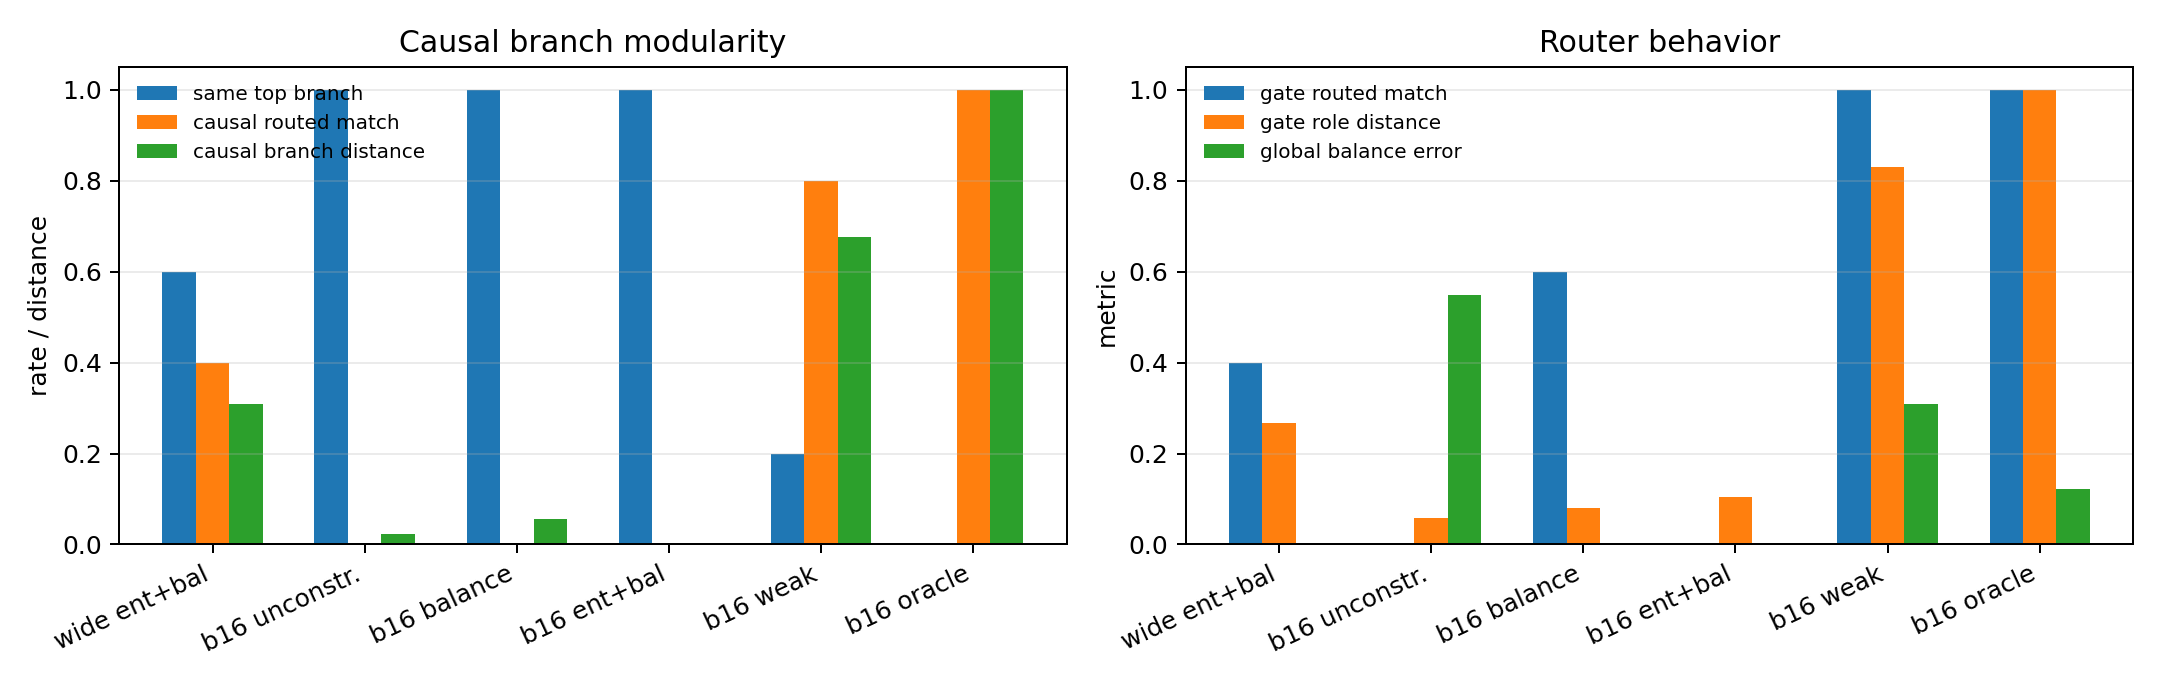
\includegraphics[width=0.92\linewidth]{figures/bottleneck16_router_comparison.png}
  \end{center}

  \vspace{-0.4em}
  \small
  Bottlenecked unlabeled routers still co-locate local and induction causally.
  Weak labels mostly work; oracle routing works perfectly.
\end{frame}

\begin{frame}{Bottlenecked Results}
  \begin{center}
  \scriptsize
  \begin{tabular}{lrrrrr}
    \toprule
    Condition & Local acc. & Ind. acc. & Same top & Routed match & Branch dist. \\
    \midrule
    \texttt{unconstrained} & 1.0000 & 0.9987 & 1.00 & 0.00 & 0.0220 \\
    \texttt{balance only} & 1.0000 & 0.9997 & 1.00 & 0.00 & 0.0551 \\
    \texttt{entropy+balance} & 1.0000 & 0.9982 & 1.00 & 0.00 & 0.0004 \\
    \texttt{weak label} & 0.9999 & 0.9991 & 0.20 & 0.80 & 0.6768 \\
    \texttt{oracle route} & 0.9999 & 1.0000 & 0.00 & 1.00 & 1.0000 \\
    \bottomrule
  \end{tabular}
  \end{center}

  \vspace{0.5em}
  All conditions solve the task, so this is not a performance failure.
\end{frame}

\begin{frame}{Comparison to Wide Branches}
  \begin{center}
  \scriptsize
  \begin{tabular}{lrr}
    \toprule
    Condition & Routed match & Branch dist. \\
    \midrule
    wide64 entropy+balance & 0.40 & 0.3082 \\
    bottleneck16 entropy+balance & 0.00 & 0.0004 \\
    wide64 weak label & 1.00 & 0.8957 \\
    bottleneck16 weak label & 0.80 & 0.6768 \\
    bottleneck16 oracle route & 1.00 & 1.0000 \\
    \bottomrule
  \end{tabular}
  \end{center}

  \vspace{0.7em}
  Shrinking branch capacity did not strengthen unlabeled modularity; if anything,
  the entropy+balance condition became cleaner co-location.
\end{frame}

\begin{frame}{Interpretation}
  \textbf{Supported:}
  \begin{itemize}
    \item 16-dim branches can support clean modularity when routing is correct.
    \item Weak role-informative routing pressure still mostly induces modularity.
  \end{itemize}

  \vspace{0.6em}
  \textbf{Not supported:}
  \begin{itemize}
    \item a simple branch-capacity bottleneck makes unlabeled entropy/balance
      regularizers discover functional modularity.
  \end{itemize}

  \vspace{0.6em}
  The bottleneck is not the missing ingredient for this toy setup.
\end{frame}

\begin{frame}{Decision}
  Do not spend the next iteration on more entropy/balance weights for the same
  task.

  \vspace{0.8em}
  Next decisive experiment:
  \begin{quote}
    Build a conflict-heavy local-vs-induction task where cohabitation is directly
    costly, then retest unlabeled routing against weak-label and oracle controls.
  \end{quote}

  \vspace{0.8em}
  Candidate variants: anti-correlated role labels, ambiguous shared-token
  layouts, or annealed weak labels that are removed after routing forms.
\end{frame}

\begin{frame}{Sources and Provenance}
  \scriptsize
  \begin{itemize}
    \item Report: \texttt{doc/phase3\_toy\_bottleneck\_router.md}
    \item Model script: \texttt{scripts/toy\_branch\_isolation\_intervention.py}
    \item Analysis script: \texttt{scripts/analyze\_bottleneck\_router\_experiment.py}
    \item Analysis output: \texttt{results/phase3\_toy\_bottleneck16\_router\_analysis/}
    \item Deck data snapshot: \texttt{presentations/2026-05-22-1609-bottleneck-router/data/}
    \item Representative command: \texttt{python3 -u scripts/toy\_branch\_isolation\_intervention.py --branch-head-dims 16}
  \end{itemize}
\end{frame}

\end{document}
